\begin{frame}{Water in Kenya}
    \centering
    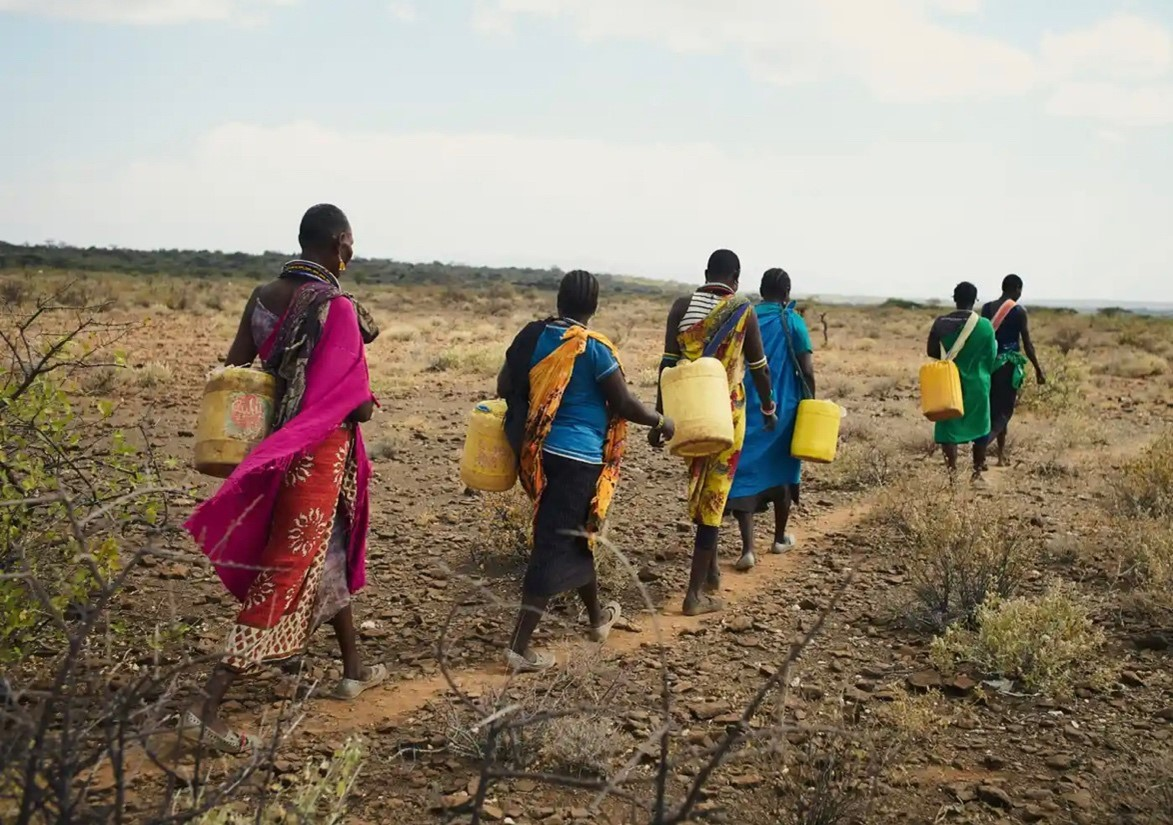
\includegraphics[width=\textwidth]{figures/kenya}
\end{frame}

\begin{frame}{Water in Kenya}
    Article 42 of the Constitution of Kenya, 2010:
    \textcolor{msred}{“Every person has the right to a clean and
    healthy environment”}, while Article43 (d) of the Constitution
    guarantees the:
    \textcolor{msred}{“Right to clean and safe water in adequate
    quantities to every person.”}
\end{frame}

\begin{frame}{Some numbers~\cite{noauthor_kenya_nodate}}
    \begin{itemize}
        \item<1-> Only about 15 percent of Kenya’s water
            resources are easily accessible, and the majority of that is
            surface water.

        \item<2-> Total abstraction 7 million m³/year - a thenth of what
            is available. Recharge is about 8\% to 9\% of total.

        \item<3-> Still over-abstracted - water level
            decline and quality deteriorates.

        \item<4-> Poor legislation and mapping - 35.000
            unregistered boreholes
    \end{itemize}
\end{frame}

\begin{frame}{Water in Kenya}
    \centering
    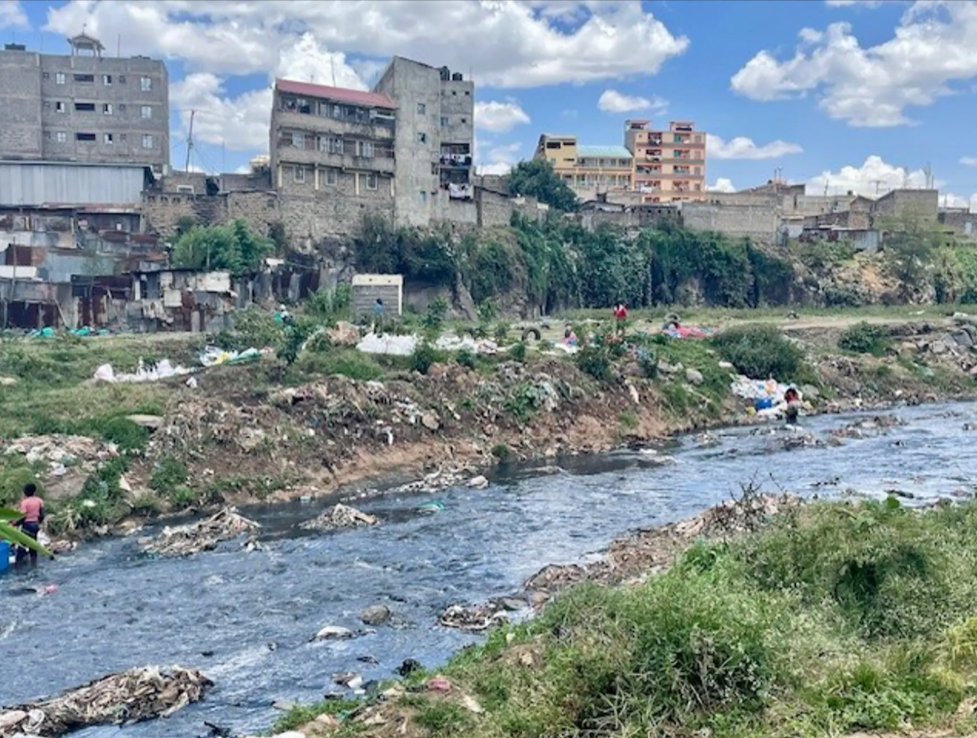
\includegraphics[width=.8\textwidth]{figures/kenyaSlum}
    \captionof*{figure}{\footnotesize Black water river running
        through the Kenyan
    slum next to Dandora landfill ©Christina Anderskov}
\end{frame}

\begin{frame}{Water in Kenya}
    Kenya generates between \textcolor{msred}{3,000 to 4,000 tons
    of waste per day.}
    \vspace{1em}

    Nairobi generates between
    \textcolor{msred}{
    2,000 to 2,500 tons of waste daily.}
    \vspace{1em}

    Less than \textcolor{msred}{half of that amount is re- or upcycled.}

    It is dumped in landfills, along roads, in streams or rivers, or burned.
    \vspace{1em}

    This happens with little awareness of the subsurface and thus
    groundwater.\footnote[frame]{\footnotesize\url{https://eng.mst.dk/about-the-danish-epa/global-cooperation/kenyacircular-economy}}

\end{frame}



\begin{frame}{Water in Ethiopia}
    \centering
    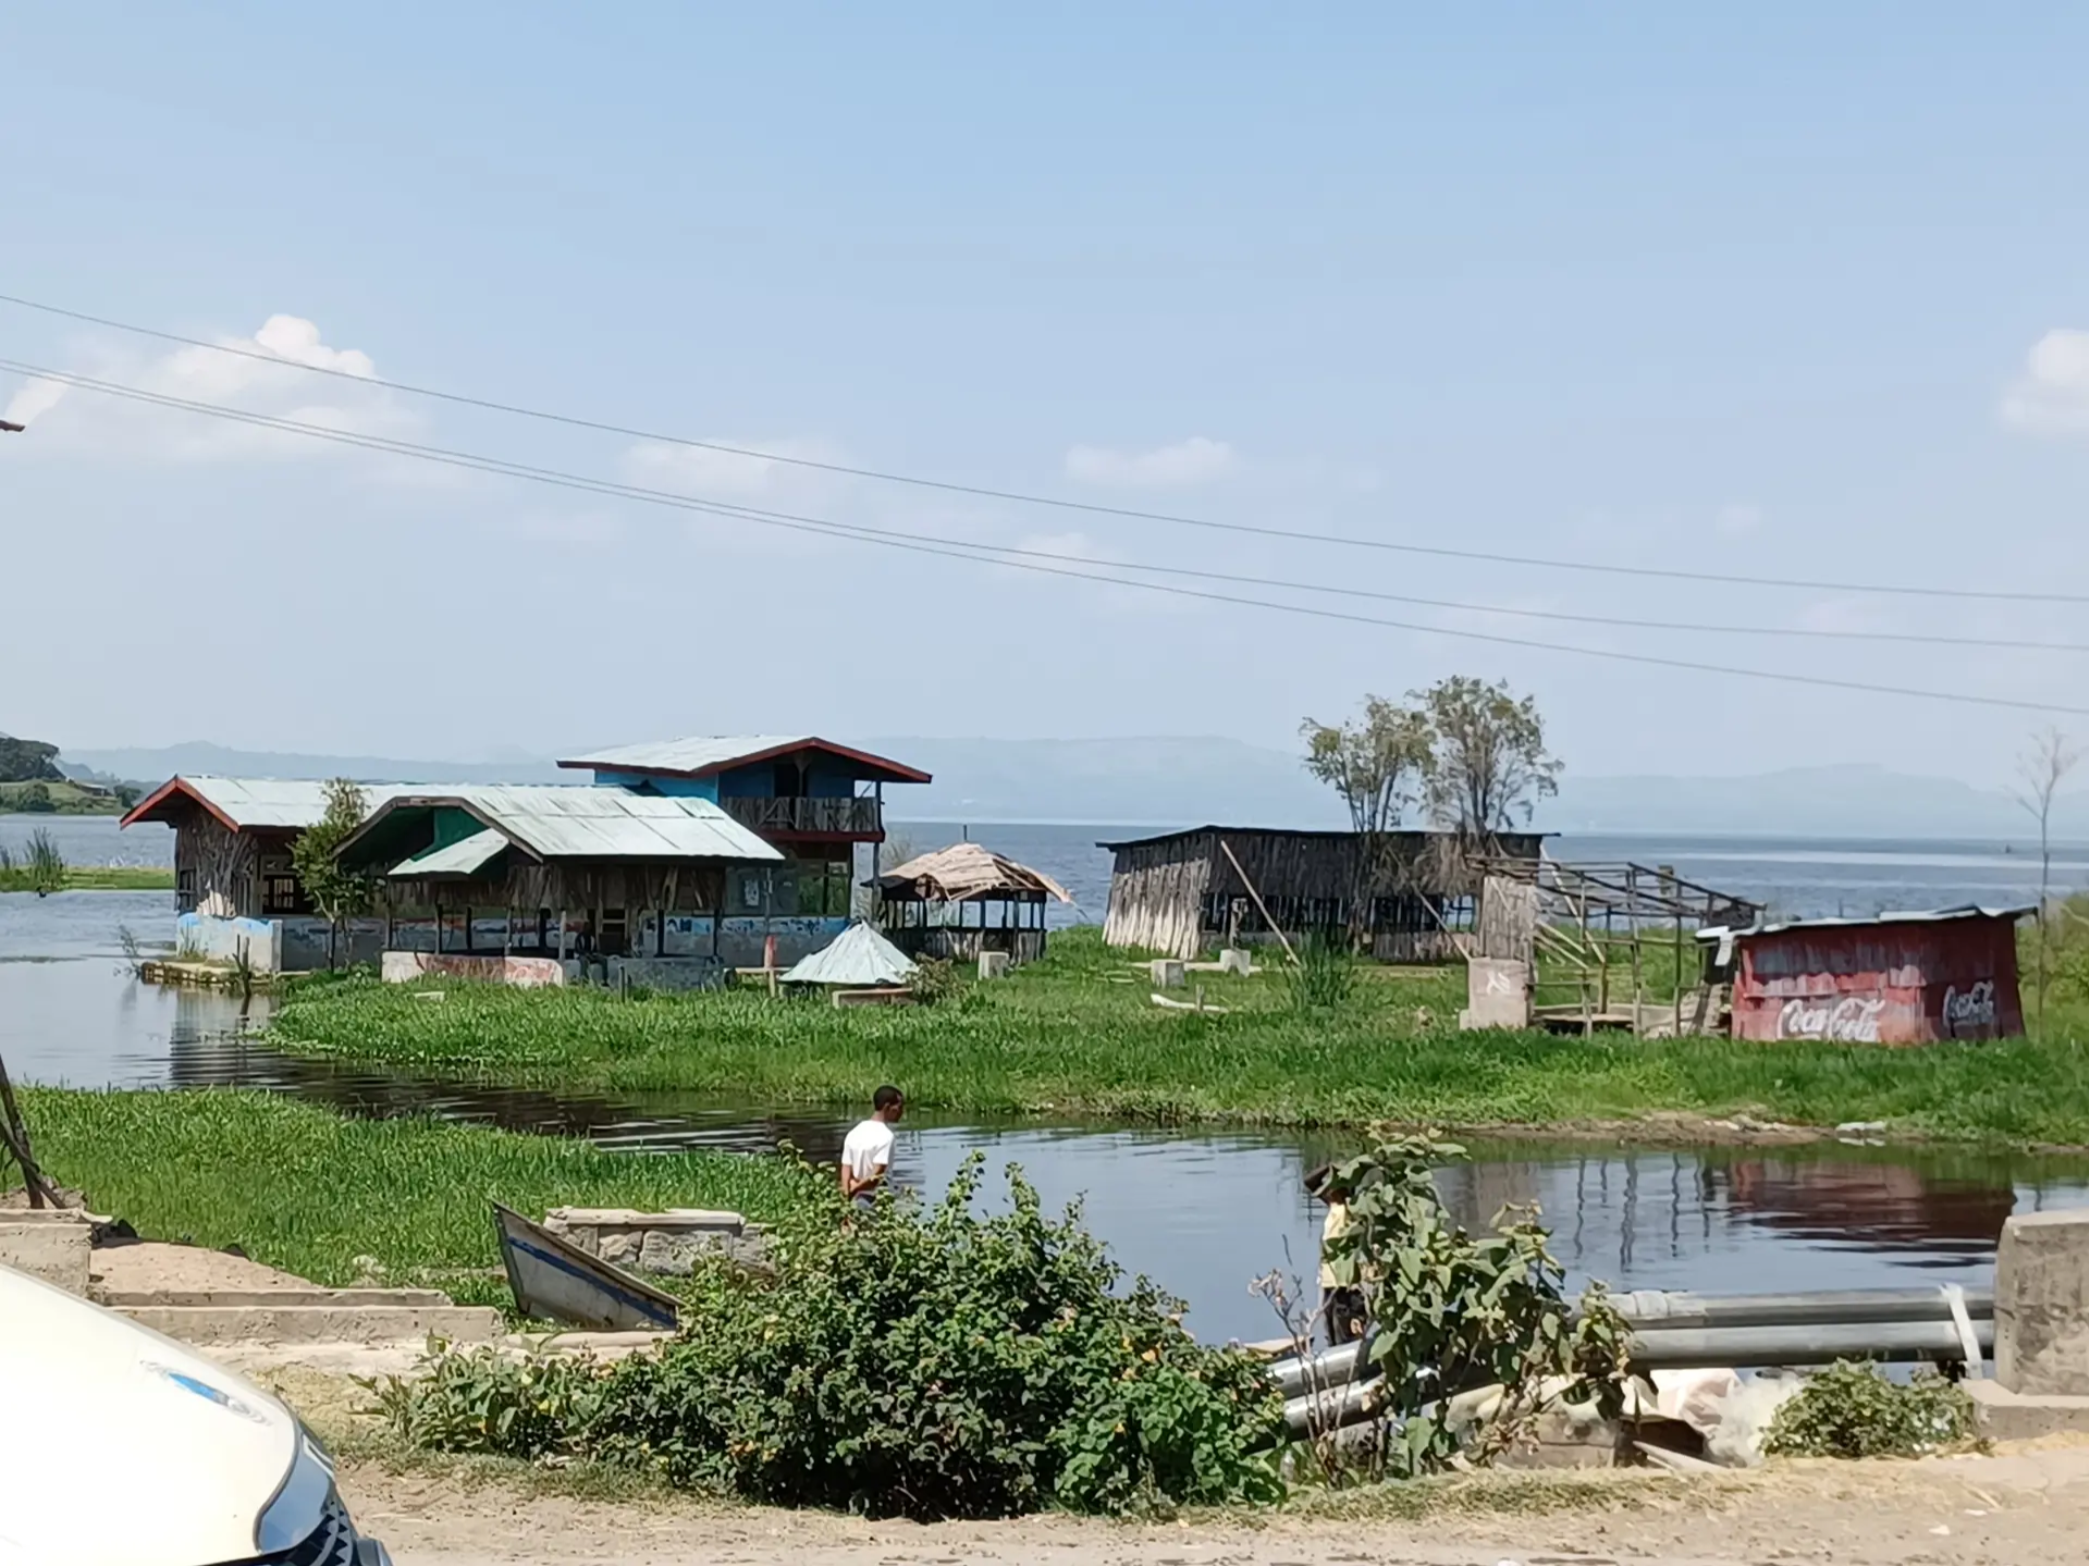
\includegraphics[width=.8\textwidth]{figures/ethiopia}
\end{frame}

\begin{frame}{Water in
    Ethiopia\footnote[frame]{\tiny\url{https://eng.mst.dk/about-the-danish-epa/global-cooperation/ethiopia}}}
    \begin{itemize}
        \item 13\% have access to safe drinking water - most of
            it from the ground.
    \end{itemize}

    Particularly impacts the rural population.

    Vast, but unevenly distributed, resources of Groundwater.
\end{frame}



\begin{frame}{EU trade with Africa}
    \centering
    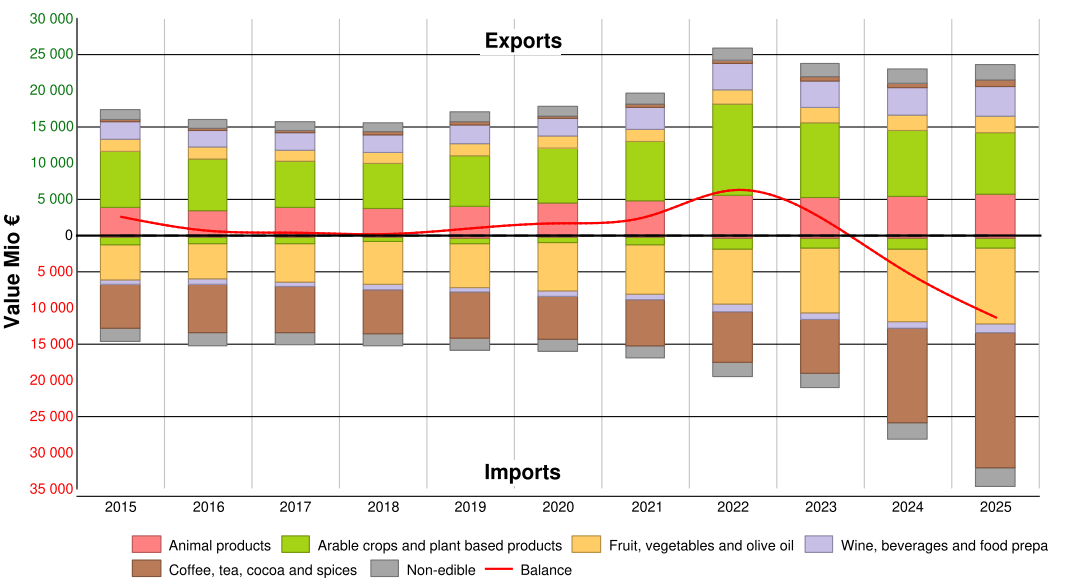
\includegraphics[width=\textwidth]{figures/africaimports}
    {Import from and exports to Africa}\footnote[frame]{Data
    from~\url{https://agriculture.ec.europa.eu/system/files/2023-05/agrifood-africa-all-countries_en.pdf}}
\end{frame}


\begin{frame}{Trade with Arfrica}
    \begin{itemize}
        \item Vast mineral exploitation by Western powers
            - Kabanga Nickel Project. No African
            representatives\footnote[frame]{\tiny\url{https://www.cetri.be/Foreign-countries-are-lining-up-to-6536?lang=fr}}.

        \item Massive farming subsidies in the EU/west outcompete local
            producers~\cite{arenas_eus_2021}.
    \end{itemize}
\end{frame}


